\documentclass[11pt,a4paper]{article}
\usepackage[russian]{babel}
\usepackage[utf8]{inputenc}
\usepackage{amsmath}
\usepackage{mathtools} 
\usepackage{amssymb}
\usepackage{multicol}
\usepackage{bm}
\usepackage{paracol}
\usepackage[hcentering, bindingoffset = 10mm, right = 15 mm, left = 15 mm, top=20mm, bottom = 20 mm]{geometry}
\newcounter{prim}
\newenvironment{prim}{%
	\addtocounter{prim}{1}
	\noindent{\\
		\textbf{\noindentПример \arabic{prim}\\}}%
}{}

\DeclareMathOperator{\tr}{\mathop{tr}}
\DeclareMathOperator{\Ker}{\mathop{Ker}}
\DeclareMathOperator{\im}{\mathop{Im}}
\DeclareMathOperator{\const}{\mathop{const}}
\DeclareMathOperator{\rg}{\mathop{rg}}
\newtheorem{definition}{Определение}[section]
\newtheorem{theorem}{Теорема}[section]
\renewcommand{\labelenumi}{\asbuk{enumi})}

\begin{document}
	\part*{Лабораторная работа 3.3.4}
	\part*{Эффект Холла в полупроводниках}
	\textbf{Работу выполнили:} \\
	{\itshape Морозов Матвей \\ Бабушкина Татьяна \\ 678 группа} \\\\
	\textbf{Цель работы:} измерение подвижности и концентрации носителей заряда в полупроводниках.
	\\\\
	\textbf{В работе используются:} электромагнит с источником питания, амперметр, миллиамперметр, милливеберметр, реостат, цифровой вольтметр, источник питания, образцы легированного германия.
	\\\\
	\part*{Экспериментальная установка}
	\begin{figure} [h!]
		\centering
		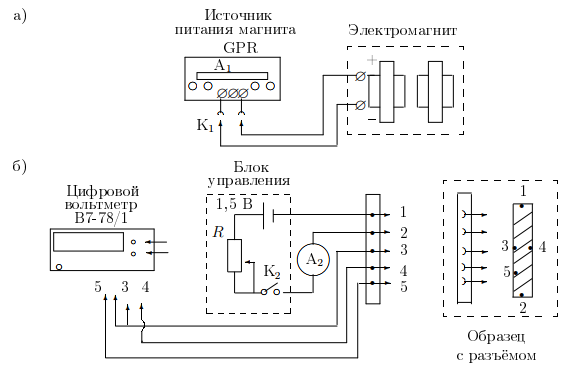
\includegraphics[width=0.6\linewidth]{6}
		\\
		\textbf {Рис. 1.} Схема установки для исследования эффекта Холла в полупроводниках \\
	\end{figure}
		
	\part*{Обработка результатов}
	
	\textbf{1)} Рассчитаем индукцию магнитного поля $B$ для каждого значения тока и построим график зависимости $B=f(I_M)$.
	\\\\
	Начальное положение милливеберметра $\Phi_0 = 2,1$ мВб.
	\\
	$SN = 75 \ \ cm^2 \text{вит}$ \\
	$\Phi = BSN \Rightarrow B = \frac{\Phi}{SN}$ \\
	$B_0 = 0,28$ Тл.
	\begin{table}[h!]
		\begin{center}
			\textbf{Таблица 1}. Зависимость $B$ от $I_M$.\\
			\begin{tabular}{|c|c|c|c|}
				\hline
				$\text{№}$  & $\Phi,\text{мВб}$ & $B,\text{Тл}$ & $I_M,A$ \\ \hline
				$\textbf{1}$ & $2,6$ & $0,34$  & $0,09$ \\ \hline
				$\textbf{2}$ & $3,3$ & $0,44$  & $0,22$ \\ \hline
				$\textbf{3}$ & $4,3$ & $0,57$  & $0,36$ \\ \hline
				$\textbf{4}$ & $5,0$ & $0,67$  & $0,46$ \\ \hline
				$\textbf{5}$ & $5,7$ & $0,76$  & $0,58$ \\ \hline
				$\textbf{6}$ & $5,9$ & $0,79$  & $0,61$ \\ \hline
				$\textbf{7}$ & $7,2$ & $0,96$  & $0,80$ \\ \hline
				$\textbf{8}$ & $7,7$ & $1,03$  & $0,91$ \\ \hline
				$\textbf{9}$ & $8,3$ & $1,11$  & $1,00$ \\ \hline
				$\textbf{10}$ & $9,1$ & $1,12$  & $1,18$ \\ \hline
				$\textbf{11}$ & $9,6$ & $1,28$  & $1,36$ \\ \hline
		\end{tabular}
\end{center}
\end{table}
\newpage
\begin{figure} [h!]
	\centering
	\textbf {График 1} \\
	Зависимость $B$ от $I_M$.\\
	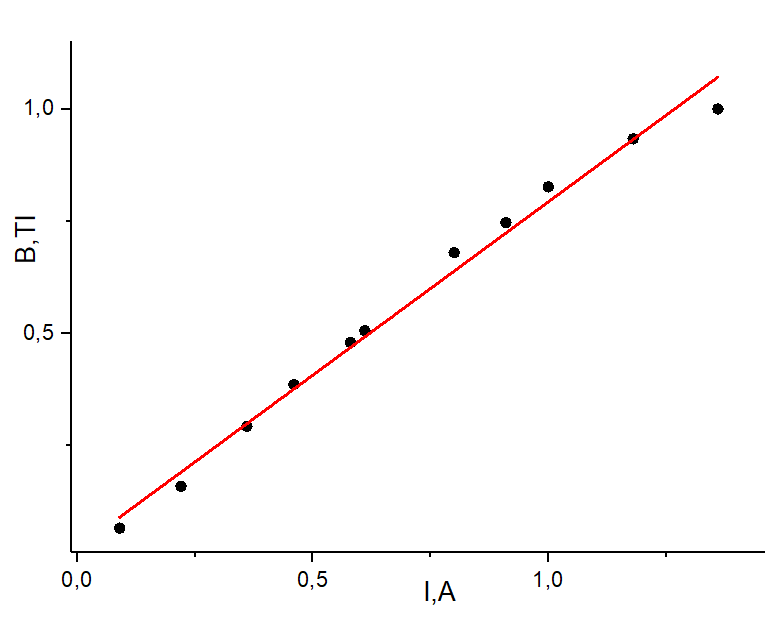
\includegraphics[width=0.6\linewidth]{1}
\end{figure}
Найдём угол наклона прямой графика $1$ при помощи метода наименьших квадратов.
\\\\
$k = \frac{<BI>}{<B^2>} \ \ \sigma k =\frac{1}{\sqrt{n}} \sqrt{\frac{<B^2>}{<I^2>} - k^2}$ \\\\
$\boxed{k=(0,77 \pm 0,03) \ \ \frac{B}{I}}$
\\\\
\textbf {2)} Рассчитаем ЭДС Холла и построим на одном графике семейство характеристик $\varepsilon_x = f(B)$ при разных значениях тока через образец. Определелим угловые коэффициенты $K(I) = \Delta \varepsilon / \Delta B$
\begin{paracol}{2}
	\begin{table}[h!]
	\begin{center}
		\textbf{Таблица 2}. \\ Зависимость $U_{34}$ от $B$ при $I_{34} = 0,3 \text{мA}$
		\\
		$U_0 = 0,011 mV$
		\\
		\begin{tabular}{|c|c|c|c|}
			\hline
			$\text{№}$  & $I_M,A$ & $B,\text{Тл}$ & $U_{34},mV$ \\ \hline
			$\textbf{1}$ & $0,05$ & $0,039$  & $0,003$ \\ \hline
			$\textbf{2}$ & $0,13$ & $0,100$  & $-0,005$ \\ \hline
			$\textbf{3}$ & $0,22$ & $0,169$  & $-0,015$ \\ \hline
			$\textbf{4}$ & $0,30$ & $0,231$  & $-0,024$ \\ \hline
			$\textbf{5}$ & $0,40$ & $0,308$  & $-0,036$ \\ \hline
			$\textbf{6}$ & $0,49$ & $0,377$  & $-0,047$ \\ \hline
			$\textbf{7}$ & $0,59$ & $0,453$  & $-0,058$ \\ \hline
			$\textbf{8}$ & $0,68$ & $0,523$  & $-0,069$ \\ \hline
			$\textbf{9}$ & $0,80$ & $0,616$  & $-0,081$ \\ \hline
			$\textbf{10}$ & $0,91$ & $0,701$  & $-0,092$ \\ \hline
			$\textbf{11}$ & $1,00$ & $0,770$  & $-0,100$ \\ \hline
			$\textbf{12}$ & $1,10$ & $0,847$  & $-0,107$ \\ \hline
			$\textbf{13}$ & $1,20$ & $0,924$  & $-0,014$ \\ \hline
			$\textbf{14}$ & $1,32$ & $1,016$  & $-0,119$ \\ \hline
			$\textbf{15}$ & $1,42$ & $1,093$  & $-0,124$ \\ \hline
			$\textbf{16}$ & $1,61$ & $1,240$  & $-0,130$ \\ \hline
		\end{tabular}
	\end{center}
\end{table}
\switchcolumn
	\begin{table}[h!]
	\begin{center}
		\textbf{Таблица 3}. \\ Зависимость $U_{34}$ от $B$ при $I_{34} = 0,4 \text{мA}$\\
		$U_0 = 0,006 mV$
		\\
		\begin{tabular}{|c|c|c|c|}
			\hline
			$\text{№}$  & $I_M,A$ & $B,\text{Тл}$ & $U_{34},mV$ \\ \hline
			$\textbf{1}$ & $0,04$ & $0,31$  & $0,001$ \\ \hline
			$\textbf{2}$ & $0,13$ & $0,10$  & $-0,011$ \\ \hline
			$\textbf{3}$ & $0,22$ & $0,17$  & $-0,024$ \\ \hline
			$\textbf{4}$ & $0,29$ & $0,22$  & $-0,035$ \\ \hline
			$\textbf{5}$ & $0,37$ & $0,28$  & $-0,047$ \\ \hline
			$\textbf{6}$ & $0,48$ & $0,37$  & $-0,065$ \\ \hline
			$\textbf{7}$ & $0,56$ & $0,43$  & $-0,077$ \\ \hline
			$\textbf{8}$ & $0,65$ & $0,50$  & $-0,091$ \\ \hline
			$\textbf{9}$ & $0,73$ & $0,56$  & $-0,102$ \\ \hline
			$\textbf{10}$ & $0,80$ & $0,62$  & $-0,111$ \\ \hline
			$\textbf{11}$ & $0,91$ & $0,70$  & $-0,125$ \\ \hline
			$\textbf{12}$ & $1,02$ & $0,79$  & $-0,138$ \\ \hline
			$\textbf{13}$ & $1,12$ & $0,86$  & $-0,147$ \\ \hline
			$\textbf{14}$ & $1,22$ & $0,94$  & $-0,155$ \\ \hline
			$\textbf{15}$ & $1,33$ & $1,02$  & $-0,162$ \\ \hline
			$\textbf{16}$ & $1,40$ & $1,08$  & $-0,166$ \\ \hline
			$\textbf{17}$ & $1,51$ & $1,16$  & $-0,171$ \\ \hline
			$\textbf{18}$ & $1,61$ & $1,24$  & $-0,176$ \\ \hline
		\end{tabular}
	\end{center}
\end{table}
\end{paracol}
\newpage
\begin{paracol}{2}
	\begin{table}[h!]
	\begin{center}
		\textbf{Таблица 4}. \\ Зависимость $U_{34}$ от $B$ при $I_{34} = 0,5 \text{мA}$\\
		$U_0 = 0,006 mV$
		\\
		\begin{tabular}{|c|c|c|c|}
			\hline
			$\text{№}$  & $I_M,A$ & $U_{34},mV$ & $B,\text{Тл}$ \\ \hline
			$\textbf{1}$ & $0,03$ & $0,000$  & $0,02$ \\ \hline
			$\textbf{2}$ & $0,09$ & $-0,008$  & $0,07$ \\ \hline
			$\textbf{3}$ & $0,16$ & $-0,021$  & $0,12$ \\ \hline
			$\textbf{4}$ & $0,24$ & $-0,036$  & $0,18$ \\ \hline
			$\textbf{5}$ & $0,33$ & $-0,053$  & $0,25$ \\ \hline
			$\textbf{6}$ & $0,42$ & $-0,071$  & $0,32$ \\ \hline
			$\textbf{7}$ & $0,51$ & $-0,087$  & $0,39$ \\ \hline
			$\textbf{8}$ & $0,60$ & $-0,105$  & $0,46$ \\ \hline
			$\textbf{9}$ & $0,71$ & $-0,124$  & $0,55$ \\ \hline
			$\textbf{10}$ & $0,82$ & $-0,144$  & $0,63$ \\ \hline
			$\textbf{11}$ & $0,91$ & $-0,158$  & $0,70$ \\ \hline
			$\textbf{12}$ & $1,01$ & $-0,172$  & $0,78$ \\ \hline
			$\textbf{13}$ & $1,09$ & $-0,183$  & $0,84$ \\ \hline
			$\textbf{14}$ & $1,21$ & $-0,193$  & $0,93$ \\ \hline
			$\textbf{15}$ & $1,31$ & $-0,202$  & $1,01$ \\ \hline
			$\textbf{16}$ & $1,42$ & $-0,209$  & $1,09$ \\ \hline
			$\textbf{17}$ & $1,53$ & $-0,216$  & $1,18$ \\ \hline
			$\textbf{18}$ & $1,60$ & $-0,220$  & $1,23$ \\ \hline
		\end{tabular}
	\end{center}
\end{table}
\switchcolumn
\begin{table}[t!] 
\begin{center} 
	\textbf{Таблица 5}. \\ Зависимость $U_{34}$ от $B$ при $I_{34} = 0,6 \text{мA}$\\
	$U_0 = 0,006 mV$
	\\
	\begin{tabular}{|c|c|c|c|} 
		\hline 
		$\text{№}$ & $I_M,A$ & $B,\text{Тл}$ & $U_{34},mV$ \\ \hline 
		$\textbf{1}$ & $0,03$ & $0,02$ & $0,000$ \\ \hline 
		$\textbf{2}$ & $0,12$ & $0,09$ & $-0,017$ \\ \hline 
		$\textbf{3}$ & $0,20$ & $0,15$ & $-0,034$ \\ \hline 
		$\textbf{4}$ & $0,30$ & $0,23$ & $-0,058$ \\ \hline 
		$\textbf{5}$ & $0,39$ & $0,30$ & $-0,080$ \\ \hline 
		$\textbf{6}$ & $0,50$ & $0,39$ & $-0,104$ \\ \hline 
		$\textbf{7}$ & $0,59$ & $0,45$ & $-0,125$ \\ \hline 
		$\textbf{8}$ & $0,66$ & $0,51$ & $-0,141$ \\ \hline 
		$\textbf{9}$ & $0,77$ & $0,59$ & $-0,162$ \\ \hline 
		$\textbf{10}$ & $0,88$ & $0,68$ & $-0,185$ \\ \hline 
		$\textbf{11}$ & $1,00$ & $0,77$ & $-0,206$ \\ \hline 
		$\textbf{12}$ & $1,23$ & $0,95$ & $-0,237$ \\ \hline 
		$\textbf{13}$ & $1,35$ & $1,04$ & $-0,249$ \\ \hline 
		$\textbf{14}$ & $1,46$ & $1,12$ & $-0,257$ \\ \hline 
		$\textbf{15}$ & $1,56$ & $1,20$ & $-0,264$ \\ \hline 
		$\textbf{16}$ & $1,59$ & $1,22$ & $-0,267$ \\ \hline 
	\end{tabular} 
\end{center} 
\end{table}
\end{paracol}
\begin{paracol}{2}
\begin{table}[t!] 
	\begin{center} 
		\textbf{Таблица 6}. \\ Зависимость $U_{34}$ от $B$ при $I_{34} = 0,7 \text{мA}$\\ 
		$U_0 = 0,008 mV$
		\\
		\begin{tabular}{|c|c|c|c|} 
			\hline 
			$\text{№}$ & $I_M,A$ & $U_{34},mV$ & $B,\text{Тл}$ \\ \hline 
			$\textbf{1}$ & $0,05$ & $-0,002$ & $0,04$ \\ \hline 
			$\textbf{2}$ & $0,11$ & $-0,018$ & $0,08$ \\ \hline 
			$\textbf{3}$ & $0,19$ & $-0,039$ & $0,15$ \\ \hline 
			$\textbf{4}$ & $0,28$ & $-0,063$ & $0,22$ \\ \hline 
			$\textbf{5}$ & $0,37$ & $-0,089$ & $0,28$ \\ \hline 
			$\textbf{6}$ & $0,46$ & $-0,114$ & $0,35$ \\ \hline 
			$\textbf{7}$ & $0,55$ & $-0,134$ & $0,42$ \\ \hline 
			$\textbf{8}$ & $0,73$ & $-0,182$ & $0,56$ \\ \hline 
			$\textbf{9}$ & $0,83$ & $-0,207$ & $0,64$ \\ \hline 
			$\textbf{10}$ & $0,93$ & $-0,230$ & $0,72$ \\ \hline 
			$\textbf{11}$ & $1,05$ & $-0,251$ & $0,81$ \\ \hline 
			$\textbf{12}$ & $1,14$ & $-0,265$ & $0,88$ \\ \hline 
			$\textbf{13}$ & $1,32$ & $-0,288$ & $1,01$ \\ \hline 
			$\textbf{14}$ & $1,42$ & $-0,298$ & $1,09$ \\ \hline 
			$\textbf{15}$ & $1,56$ & $-0,310$ & $1,20$ \\ \hline 
			$\textbf{16}$ & $1,59$ & $-0,312$ & $1,22$ \\ \hline 
		\end{tabular} 
	\end{center} 
\end{table}
\switchcolumn
\begin{table}[h!] 
	\begin{center} 
		\textbf{Таблица 7}. \\ Зависимость $U_{34}$ от $B$ при $I_{34} = 0,8 \text{мA}$\\ 
		$U_0 = 0,009 mV$
		\\
		\begin{tabular}{|c|c|c|c|} 
			\hline 
			$\text{№}$ & $I_M,A$ & $B,\text{Тл}$ & $U_{34},mV$ \\ \hline 
			$\textbf{1}$ & $0,03$ & $0,02$ & $0,003$ \\ \hline 
			$\textbf{2}$ & $0,15$ & $0,12$ & $-0,034$ \\ \hline 
			$\textbf{3}$ & $0,23$ & $0,18$ & $-0,057$ \\ \hline 
			$\textbf{4}$ & $0,32$ & $0,25$ & $-0,084$ \\ \hline 
			$\textbf{5}$ & $0,41$ & $0,32$ & $-0,011$ \\ \hline 
			$\textbf{6}$ & $0,48$ & $0,37$ & $-0,132$ \\ \hline 
			$\textbf{7}$ & $0,58$ & $0,45$ & $-0,161$ \\ \hline 
			$\textbf{8}$ & $0,68$ & $0,52$ & $-0,192$ \\ \hline 
			$\textbf{9}$ & $0,74$ & $0,57$ & $-0,209$ \\ \hline 
			$\textbf{10}$ & $0,82$ & $0,63$ & $-0,229$ \\ \hline 
			$\textbf{11}$ & $0,91$ & $0,70$ & $-0,253$ \\ \hline 
			$\textbf{12}$ & $0,98$ & $0,75$ & $-0,274$ \\ \hline 
			$\textbf{13}$ & $1,07$ & $0,82$ & $-0,291$ \\ \hline 
			$\textbf{14}$ & $1,22$ & $0,94$ & $-0,313$ \\ \hline 
			$\textbf{15}$ & $1,37$ & $1,05$ & $-0,331$ \\ \hline 
			$\textbf{16}$ & $1,48$ & $1,14$ & $-0,342$ \\ \hline
			$\textbf{17}$ & $1,58$ & $1,22$ & $-0,351$ \\ \hline 
		\end{tabular} 
	\end{center} 
\end{table}
\end{paracol}
\newpage
\begin{paracol}{2}
\begin{table}[h!] 
	\begin{center} 
		\textbf{Таблица 8}. \\ Зависимость $U_{34}$ от $B$ при $I_{34} = 0,9 \text{мA}$\\ 
		$U_0 = 0,010 mV$
		\\
		\begin{tabular}{|c|c|c|c|} 
			\hline 
			$\text{№}$ & $I_M,A$ & $B,\text{Тл}$ & $U_{34},mV$ \\ \hline 
			$\textbf{1}$ & $0,05$ & $0,04$ & $-0,006$ \\ \hline 
			$\textbf{2}$ & $0,15$ & $0,12$ & $-0,035$ \\ \hline 
			$\textbf{3}$ & $0,24$ & $0,18$ & $-0,069$ \\ \hline 
			$\textbf{4}$ & $0,33$ & $0,25$ & $-0,100$ \\ \hline 
			$\textbf{5}$ & $0,42$ & $0,32$ & $-0,132$ \\ \hline 
			$\textbf{6}$ & $0,54$ & $0,42$ & $-0,179$ \\ \hline 
			$\textbf{7}$ & $0,64$ & $0,49$ & $-0,205$ \\ \hline 
			$\textbf{8}$ & $0,77$ & $0,59$ & $-0,249$ \\ \hline 
			$\textbf{9}$ & $0,87$ & $0,67$ & $-0,279$ \\ \hline 
			$\textbf{10}$ & $1,01$ & $0,78$ & $-0,317$ \\ \hline 
			$\textbf{11}$ & $1,10$ & $0,85$ & $-0,336$ \\ \hline 
			$\textbf{12}$ & $1,20$ & $0,92$ & $-0,355$ \\ \hline 
			$\textbf{13}$ & $1,32$ & $1,02$ & $-0,372$ \\ \hline 
			$\textbf{14}$ & $1,45$ & $1,12$ & $-0,388$ \\ \hline 
			$\textbf{15}$ & $1,53$ & $1,18$ & $-0,397$ \\ \hline 
			$\textbf{16}$ & $1,57$ & $1,21$ & $-0,402$ \\ \hline 
		\end{tabular} 
	\end{center} 
\end{table}
\switchcolumn
\begin{table}[h!] 
	\begin{center} 
		\textbf{Таблица 9}. \\ Зависимость $U_{34}$ от $B$ при $I_{34} = 1 \text{мA}$\\ 
		$U_0 = 0,011 mV$
		\\
		\begin{tabular}{|c|c|c|c|} 
			\hline 
			$\text{№}$ & $I_M,A$ & $B,\text{Тл}$ & $U_{34},mV$ \\ \hline 
			$\textbf{1}$ & $0,07$ & $0,05$ & $-0,013$ \\ \hline 
			$\textbf{2}$ & $0,15$ & $0,12$ & $-0,042$ \\ \hline 
			$\textbf{3}$ & $0,24$ & $0,18$ & $-0,075$ \\ \hline 
			$\textbf{4}$ & $0,33$ & $0,25$ & $-0,109$ \\ \hline 
			$\textbf{5}$ & $0,40$ & $0,31$ & $-0,139$ \\ \hline 
			$\textbf{6}$ & $0,50$ & $0,39$ & $-0,177$ \\ \hline 
			$\textbf{7}$ & $0,59$ & $0,45$ & $-0,211$ \\ \hline 
			$\textbf{8}$ & $0,70$ & $0,54$ & $-0,251$ \\ \hline 
			$\textbf{9}$ & $0,80$ & $0,62$ & $-0,291$ \\ \hline 
			$\textbf{10}$ & $0,91$ & $0,70$ & $-0,321$ \\ \hline 
			$\textbf{11}$ & $1,02$ & $0,79$ & $-0,356$ \\ \hline 
			$\textbf{12}$ & $1,13$ & $0,87$ & $-0,381$ \\ \hline 
			$\textbf{13}$ & $1,22$ & $0,94$ & $-0,398$ \\ \hline 
			$\textbf{14}$ & $1,32$ & $1,02$ & $-0,413$ \\ \hline 
			$\textbf{15}$ & $1,50$ & $1,16$ & $-0,438$ \\ \hline 
			$\textbf{16}$ & $1,57$ & $1,21$ & $-0,445$ \\ \hline 
		\end{tabular} 
	\end{center} 
\end{table}
\end{paracol}
$\varepsilon_x = U_{34} + U_0$
\begin{figure}[h!]
	\centering
		\textbf {График 2} \\
	Семейство характеристик $\varepsilon_x = f(B)$ при разных значениях тока через образец\\
	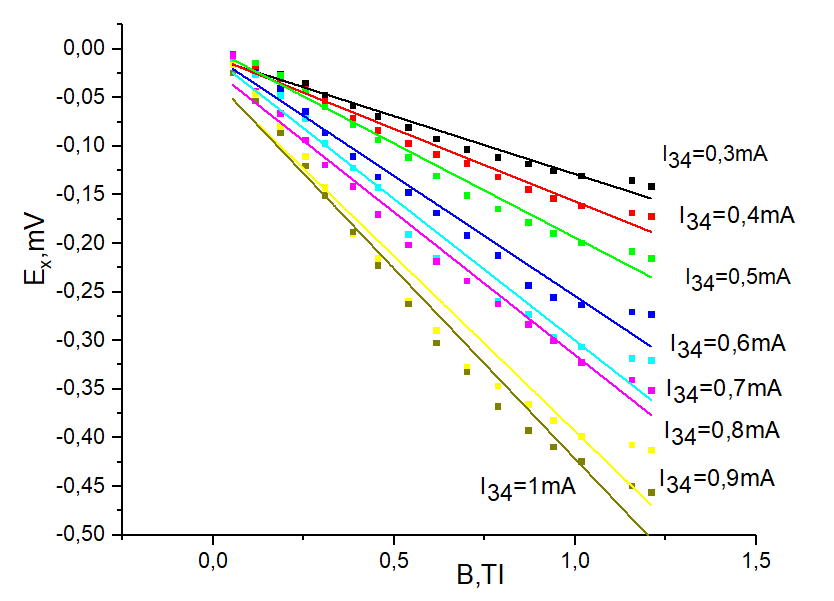
\includegraphics[width=0.8\linewidth]{3}
\end{figure}
\\
Определим угловые коэффициенты $K(I)$ при помощи метода наименьших квадратов.
\\\\
$k = \frac {<\varepsilon_x B> - <\varepsilon_x><b>}{<B^2>-<B>^2}, \ \ \delta k = \frac{1}{\sqrt{n}} \sqrt{\frac{<\varepsilon_x^2>-<\varepsilon_x>^2}{<B^2>-<B>^2} - k^2}$
\\\\
и занесём их в таблицу $10$.
\newpage
\begin{table}[h!] 
	\begin{center} 
		\textbf{Таблица 10}. \\ Зависимость $K$ от $I_{34}$\\
		\begin{tabular}{|c|c|c|c|} 
			\hline 
			$\text{№}$ & $k,\text{мВ/Тл}$ & $\delta k,\text{мВ/Тл}$ & $I_{34},A$ \\ \hline 
			$\textbf{1}$ & $-0,119$ & $0,005$ & $0,3$ \\ \hline
			$\textbf{2}$ & $-0,149$ & $0,006$ & $0,4$ \\ \hline
			$\textbf{3}$ & $-0,194$ & $0,007$ & $0,5$ \\ \hline
			$\textbf{4}$ & $-0,247$ & $0,011$ & $0,6$ \\ \hline
			$\textbf{5}$ & $-0,291$ & $0,014$ & $0,7$ \\ \hline
			$\textbf{6}$ & $-0,294$ & $0,011$ & $0,8$ \\ \hline
			$\textbf{7}$ & $-0,361$ & $0,022$ & $0,9$ \\ \hline
			$\textbf{8}$ & $-0,392$ & $0,017$ & $1,0$ \\ \hline
		\end{tabular} 
	\end{center} 
\end{table}
\textbf{3)} Построим график $K=f(I)$.\\
\begin{figure}[h!]
	\centering
	\textbf {График 3} \\
	Зависимость $K$ от $I_{34}$\\
	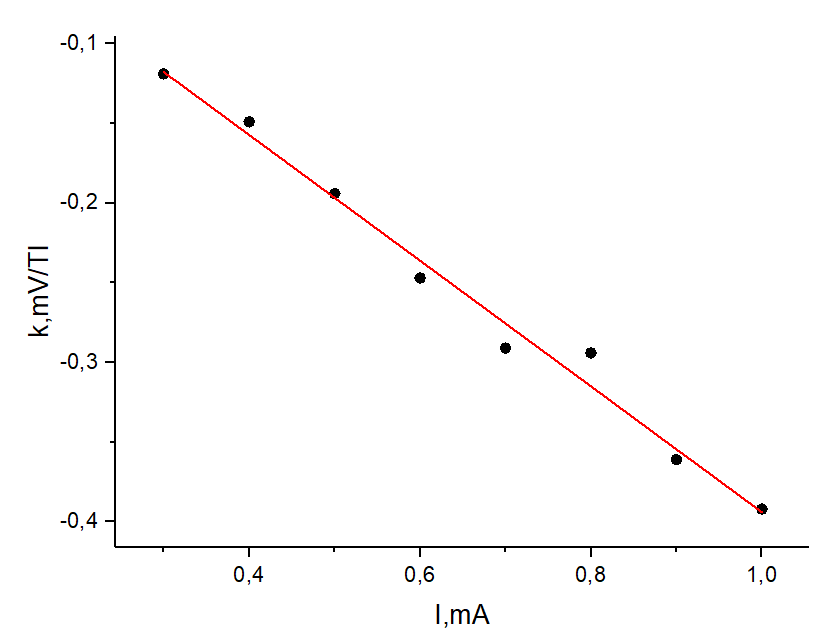
\includegraphics[width=0.7\linewidth]{4}
\end{figure}
\\
С помощью МНК рассчитали тангенс наклона прямой графика $3$. \\\\ $k^{'} = (-0,395 \pm 0,019) \frac{\text{В}}{\text{А Тл}}$ \\\\
Рассчитаем величину постоянной Холла $R_x$ с помощью формулы $\varepsilon_x= -R_x \frac{IB}{a}$.
\\\\
$R_x = - \varepsilon_x \frac{a}{IB} = k^{'} \cdot a$, где $a = 1,5 mm$ \\\\
$\boxed{R_x = (5,92 \pm 0,29) \cdot 10^{-4} \ \  \frac{\text{м}^3}{\text{Кл}}}$
\\\\
\textbf{4)} Рассчитаем концентрацию $n$ носителей тока в образце по формуле $R_x = \cfrac{1}{ne}$.
\\\\
$n = \cfrac{1}{R_x\cdot e}$
\\\\
$\boxed{n = (1,06 \pm 0,07) \cdot 10^{22} \frac{1}{\text{м}^{3}}}$
\\\\
\textbf{5)} Рассчитаем удельную проводимость $\sigma$ материала образца по формуле $\sigma = \cfrac{I L_{35}}{U_{35}al}$ \\\\
$L_{35} = 3 \ \  mm$, 
$U_{35} = 1,696 \ \ mV$ \\
$a = 1,5 \ \ mm$,
$l = 1,7 \ \ mm$, $I = 1 \ \ mA$
\\\\
$\boxed{\sigma = (6,93 \pm 0,41) \cdot 10^3 \ \ \frac{A}{\text{В м}}}$
\\\\
\textbf{6)} Используя найденные значения концентрации $n$ и проводимости $\sigma$, с помощью формулы $\sigma = e \cdot n \cdot b$ вычислим подвижность $b$ носителей тока. \\\\
$b = \cfrac {\sigma}{ne}$
\\\\
$\delta b = b \cdot \sqrt{(\frac{\delta \sigma}{\sigma})^2 +\frac{\delta n}{n})^2 }$
\\\\
$\boxed{b = (4,09 \pm 0,36) \cdot 10^3 \ \ \frac{\text{м}^2}{Bc}}$
\part*{Вывод}
\begin{enumerate}
	\item Исследовали эффект Холла а образце из германия, нашли для него постоянную Холла \\
	$\boxed{R_x = (5,92 \pm 0,29) \cdot 10^{-4} \ \  \frac{\text{м}^3}{\text{Кл}}}$
	\item Измерили концентрацию носителей заряда в образце.\\
	$\boxed{n = (1,06 \pm 0,07) \cdot 10^{22} \frac{1}{\text{м}^{3}}}$
	\item Определили, что носителями являются электроны и вычислили их подвижность\\
	$\boxed{\sigma = (6,93 \pm 0,41) \cdot 10^3 \ \ \frac{A}{\text{В м}}}$
\end{enumerate}



\end{document}